\documentclass[10pt, a5paper]{article}
\usepackage{pdfpages}
\usepackage{parallel}
\usepackage[T2A]{fontenc}
\usepackage{ucs}
\usepackage[utf8x]{inputenc}
\usepackage[polish,english,russian]{babel}
\usepackage{hyperref}
\usepackage{rotating}
\usepackage[inner=2cm,top=1.8cm,outer=2cm,bottom=2.3cm,nohead]{geometry}
\usepackage{listings}
\usepackage{graphicx}
\usepackage{wrapfig}
\usepackage{longtable}
\usepackage{indentfirst}
\usepackage{array}
\newcolumntype{P}[1]{>{\raggedright\arraybackslash}p{#1}}
\frenchspacing
\usepackage{fixltx2e} %text sub- and superscripts
\usepackage{icomma} % коскі ў матэматычным рэжыме
\PreloadUnicodePage{4}

\newcommand{\longpage}{\enlargethispage{\baselineskip}}
\newcommand{\shortpage}{\enlargethispage{-\baselineskip}}

\def\switchlang#1{\expandafter\csname switchlang#1\endcsname}
\def\switchlangbe{
\let\saverefname=\refname%
\def\refname{Літаратура}%
\def\figurename{Іл.}%
}
\def\switchlangen{
\let\saverefname=\refname%
\def\refname{References}%
\def\figurename{Fig.}%
}
\def\switchlangru{
\let\saverefname=\refname%
\let\savefigurename=\figurename%
\def\refname{Литература}%
\def\figurename{Рис.}%
}

\hyphenation{admi-ni-stra-tive}
\hyphenation{ex-pe-ri-ence}
\hyphenation{fle-xi-bi-li-ty}
\hyphenation{Py-thon}
\hyphenation{ma-the-ma-ti-cal}
\hyphenation{re-ported}
\hyphenation{imp-le-menta-tions}
\hyphenation{pro-vides}
\hyphenation{en-gi-neering}
\hyphenation{com-pa-ti-bi-li-ty}
\hyphenation{im-pos-sible}
\hyphenation{desk-top}
\hyphenation{elec-tro-nic}
\hyphenation{com-pa-ny}
\hyphenation{de-ve-lop-ment}
\hyphenation{de-ve-loping}
\hyphenation{de-ve-lop}
\hyphenation{da-ta-ba-se}
\hyphenation{plat-forms}
\hyphenation{or-ga-ni-za-tion}
\hyphenation{pro-gramming}
\hyphenation{in-stru-ments}
\hyphenation{Li-nux}
\hyphenation{sour-ce}
\hyphenation{en-vi-ron-ment}
\hyphenation{Te-le-pathy}
\hyphenation{Li-nux-ov-ka}
\hyphenation{Open-BSD}
\hyphenation{Free-BSD}
\hyphenation{men-ti-on-ed}
\hyphenation{app-li-ca-tion}

\def\progref!#1!{\texttt{#1}}
\renewcommand{\arraystretch}{2} %Іначай формулы ў матрыцы зліпаюцца з лініямі
\usepackage{array}

\def\interview #1 (#2), #3, #4, #5\par{

\section[#1, #3, #4]{#1 -- #3, #4}
\def\qname{LVEE}
\def\aname{#1}
\def\q ##1\par{{\noindent \bf \qname: ##1 }\par}
\def\a{{\noindent \bf \aname: } \def\qname{L}\def\aname{#2}}
}

\def\interview* #1 (#2), #3, #4, #5\par{

\section*{#1\\{\small\rm #3, #4. #5}}

\def\qname{LVEE}
\def\aname{#1}
\def\q ##1\par{{\noindent \bf \qname: ##1 }\par}
\def\a{{\noindent \bf \aname: } \def\qname{L}\def\aname{#2}}
}

\begin{document}
\title{Smart GreenHouse}
\author{Dzmitry Yasevich, Vasili Slapik, Pavel Vervenko, \\
Dmitry Ogievich --- Minsk, Belarus\footnote{\url{dzmitry_yasevich@epam.com}, \url{http://lvee.org/ru/abstracts/131}}}
\maketitle
\begin{abstract}
«Java for Farmers»: Greenhouse monitoring and automation, using Java, Raspberry Pi, Linux and multiple sensors. Smart Greenhouse Project is a Oracle IoT winner 2014 in professional category.
\end{abstract}
\subsection*{История проекта}

Ни для кого не секрет, что ``умные'' программные решения (дома, парники, и т.д.) находят все большее применение в реальном мире. Узнав о существовании Java Embedded для создания ``Интернета вещей'', мы загорелись идеей попробовать ее в деле. После недолгого обсуждения в качестве объекта для экспериментов была выбрана ``умная'' теплица.

Причин было несколько. Первая из них --- умными домами занимаются широкий круг инженеров и энтузиастов, начиная от студенческих клубов и заканчивая серьезными IT-компаниями, поэтому здесь было тяжело создать что-то действительно новое и интересное.

Вторая, но не менее значимая причина, заключается в том, что Беларусь --- это страна, в которой хорошо развит аграрный сектор. Наша команда решила быть патриотичной и создать устройство достаточно простое, но при этом потенциально полезное для использования в сельском хозяйстве. Таким образом выбор пал на теплицу, как точку приложения наших сил.

\subsection*{Java Embedded}

Java уже успела зарекомендовать себя в качестве успешной платформы для решения множества задач, включая и ``умные'' системы. Если охватывать весь спектр техники, то можно насчиать более 10 млрд устройств, использующих Java. При этом подавляющая часть таких устройств так или иначе базируются на *nix платформах.

Почему все-таки стоит использовать Java для встраиваемых систем; ведь на первый взгляд у Java недостатков гораздо больше, чем преимуществ:

\begin{itemize}
  \item Java является одной из самых популярных платформ для разработки приложений;
  \item Оптимизирована для Embedded решений;
  \item Высокопроизводительные, переносимые приложения;
  \item Свободно распространяемые инструменты разработчика;
  \item Проверенная модель безопасности.
\end{itemize}

Как показала практика, для создания ``умной'' теплицы с помощью Java Embedded достаточно скромных ресурсов Raspberry Pi, работающей под управлением Linux.

\subsection*{Функциональные возможности теплицы}

К числу основных особенностей проекта относятся:

\begin{itemize}
  \item Контроль и управление светом.
  \item Контроль полива.
  \item Контроль температуры и влажности.
  \item Удаленный мониторинг текущего состояния теплицы.
  \item Автоматическое управление теплицей.
  \item Автоматический процесс фотографирования роста растений.
  \item Низкая потребляемая мощность.
  \item Защита от коротких замыканий и отключения электричества.
\end{itemize}

Таким образом, наша разработка на данный момент представляет собой полнофункциональную автоматизированную систему, которая позволяет выращивать комнатные растения, сохраняя душевное спокойствие владельца теплицы. Обеспечивается удаленное управление и мониторинг света, температуры и влажности. Также запланирована возможность дистанционной проверки текущего процесса роста в режиме онлайн.

\subsection*{Реализация}

При создании нашего проекта мы старались использовать открытые и свободные компоненты и технологии: Raspberry Pi, Java Embedded, Raspbian, pi4j, Jetty и нескольких сенсоров.

Электрическая схема Smart GreenHouse показана на рисунке.

\begin{figure}[h!]
  \centering
  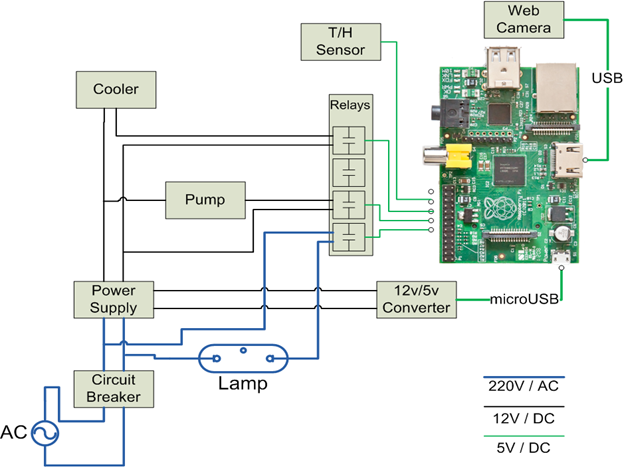
\includegraphics[scale=0.8]{13_2014_1.png}
\end{figure}

Raspbian --- это операционная система, основанная на Debian и оптимизированная для Raspberry Pi, а pi4j --- библиотека для работы с аппаратной частью Raspberry Pi.

Ниже приведен пример кода на Java для датчика влажности и температуры при использовании pi4j:

\begin{verbatim}
// инициализация
GpioController gpio = GpioFactory.getInstance();
GpioPinDigitalOutput light = gpio.provisionDigitalOutputPin(
	RaspiPin.GPIO_07, "Light", PinState.LOW); 
	// подключились к пину 7
	
light.setShutdownOptions(true, PinState.LOW, 
	PinPullResistance.OFF); /* задали опцию, чтоб на выходе 
	из приложения этот пин отключался (чтоб свет гас) */

// управление
light.high(); // включить пин
light.low(); // выключить
\end{verbatim}
\subsection*{Текущий статус и планы}

На данный момент проект все еще развивается --- добавляем поддержку разных датчиков, решаем проблемы, возникающие при совместной работе нескольких таких устройств. 
Также создаем специализированный дистрибутив на базе Yocto Project, содержащий все необходимое для работы автоматизированной теплицы ``из коробки''.

Полный исходный код управляющей части проекта доступен по адресу \url{https://bitbucket.org/Temdegon/greenhouse}

\end{document}
